\chapter{Analyse}\label{analyse}

In diesem Kapitel werden die vorgestellten Daten näher untersucht. Das beinhaltet sowohl die Anwendung der in Kapitel \ref{artefakterkennung} beschriebenen existierenden Verfahren als auch eine Analyse der verwendeten Merkmale.

\section{Aufbau und Evaluation der Verfahren}

Um Modelle zur Beurteilung der Signalqualität anzuwenden und zu untersuchen, müssen sowohl die verwendeten Merkmale extrahiert als auch die Ergebnisse evaluiert werden. In den hier durchgeführten Untersuchungen wurde die Segmentlänge standardmäßig auf 10\,Sekunden festgelegt und der Abstand der Segmente auf 1\,Sekunde, wodurch sich die Segmente zu je 90\,\% überlappen. Diese Segmentlänge wird zum einen häufiger verwendet\footcite[Vgl.][]{Yu2020, Sadek2016, Orphanidou2015}, zum anderen bietet sie eine ausreichend große Robustheit für die Annotation der Daten. Die für die Verfahren jeweils benötigten Merkmale werden segmentweise extrahiert und serialisiert. Zusätzlich zu den verwendeten Merkmalen werden allgemeine Informationen über die Segmente gespeichert. Dazu gehören Patient*innen-ID, EKG-Herzrate, BKG-Herzrate, absoluter und relativer Fehler, $E\textsubscript{HR}$ und die binäre Annotation. Für letztere wird als Standard $E\textsubscript{HR} = 10$ als Schwellwert verwendet.

Diese Daten werden anschließend in Trainings- und Validierungsset aufgeteilt. Um diese beiden Gruppen inhaltlich vollständig zu trennen und auszuschließen, dass auf teilweise bekannten Daten validiert wird, geschieht die Trennung anhand der Patient*innen-IDs, sodass Segmente einer Person lediglich in einem der beiden Sets verwendet werden. Das Validierungsset in dieser Arbeit entspricht einem Drittel der Patient*innen, die restlichen zwei Drittel werden zur Datenexploration, zur Merkmalskonstruktion und zum Training verwendet. Die Verteilung von $E\textsubscript{HR}$ im Validierungsset ist in Abbildung \ref{fig:validation-set} gezeigt. Von den existierenden Verfahren benötigen zwei keine Trainingsphase; um vergleichbare Ergebnisse zu erhalten, wird auch bei diesen bei der Evaluation nur das Validierungsset betrachtet.

\begin{figure}[H]
	\centering
	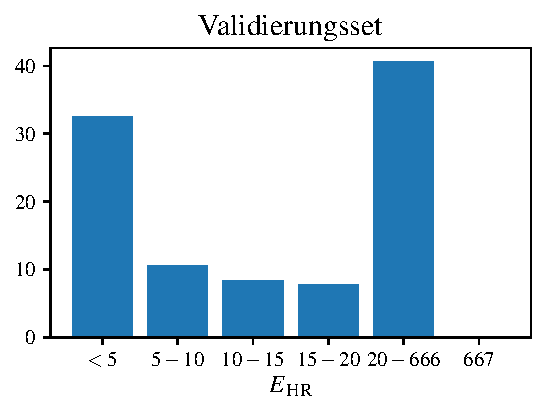
\includegraphics{pic/mlp-statistical-testset.pdf}
	\caption[Verteilung von $E\textsubscript{HR}$ auf dem Validierungsset]{Verteilung von $E\textsubscript{HR}$ auf dem Validierungsset}
	\label{fig:validation-set}
\end{figure}


Wie schon in Kapitel \ref{artefakterkennung} beschrieben, sind bei der Verarbeitung von medizinischen Signalen zwei Bereiche wichtig: Die Coverage und die Qualität des Signals, in diesem Fall also die Genauigkeit der geschätzten Herzrate im Vergleich zur Referenz. Diese beiden müssen gegeneinander aufgewogen werden und werden aus diesem Grund beide betrachtet. Die Qualität der Modelle kann zunächst anhand der binären Klassifikation beurteilt werden. Da diese aber keine Auskunft darüber enthält, wie nah klassifiziertes Signal an dem Schwellwert für $E\textsubscript{HR}$ liegt, wird letzteres in einer tiefergehenden Evaluation ebenfalls betrachtet. Im Zuge dessen wird sowohl der Fehler auf dem als informativ klassifizierten Signal betrachtet als auch die Coverage in Bezug auf das ganze Signal für verschiedene Fehlergrößen. Insbesondere falsch klassifiziertes Signal, also Falsch-Negative und Falsch-Positive, ist interessant, um zu beurteilen, ob Fehlklassifikationen lediglich im Grenzbereich $E\textsubscript{HR} \approx 10$ oder allgemein vorkommen.

\section{Anwendung existierender Verfahren}

Zunächst werden die in Kapitel \ref{artefakterkennung} beschriebenen existierenden Artefakterkennungsverfahren mit den in dieser Arbeit untersuchten Daten wie oben beschrieben getestet und ihre Leistungsfähigkeit untersucht und bewertet.

\subsection{Ähnlichkeit der Intervallschätzer des CLIE-Algorithmus}

Der \ac{SQI}, der die Ähnlichkeit der Intervallschätzer des \ac{CLIE}-Algorithmus angibt, wird im Normalfall herzschlagweise angewendet. Da die Datenannotion nur bereichsweise vorgenommen werden kann, wurde entschieden, ein Segment als informativ zu klassifizieren, wenn mit den Herzschlägen, deren \ac{SQI} über einem Schwellwert $q_{th}$ liegt, eine Coverage über einem gegebenen Schwellwert $c_{th}$ auf dem Segment erreicht wird. %TODO: evtl kürzen/trennen
Getestete Schwellwerte für die Coverage sind 50\,\%, 75\,\% und 100\,\%. Zum Testen des Algorithmus wurde unter anderem $q_{th} = 0{,}4$ gewählt, da dieser Wert auch von \citeauthor{Zink2017} verwendet wird.\footcite[]{Zink2017} Zusätzlich wurden $q_{th} = 0{,}3$ und $q_{th} = 0{,}2$ untersucht, um den Einfluss von $q_{th}$ einzuordnen. Bei der Berechnung der Merkmale werden für jedes Segment die detektierten Herzschläge extrahiert, deren \ac{SQI} über $q_{th}$ liegt. Auf Basis dieser Intervalllängen wird wie in Kapitel \ref{annotation} beschrieben die Herzrate, im Folgenden $HR\textsubscript{SQI}$ genannt, ermittelt. Extrahierte Merkmale sind damit in diesem Fall $HR\textsubscript{SQI}$ und die Coverage $C\textsubscript{SQI}$. Für die Auswertung muss beachtet werden, dass sich die ermittelte Herzrate $HR\textsubscript{SQI}$ von der zur Annotation verwendeten Herzrate unterscheidet. Aufgrund der Vergleichbarkeit wird $HR\textsubscript{SQI}$ nicht für die Berechnung des \ac{MAE} des Algorithmus verwendet.

Bei einer ersten Betrachtung von \ac{MAE}, Coverage und Accuracy wird sichtbar, dass die Wahl der Schwellwerte großen Einfluss auf das Ergebnis hat und in jedem Fall Aussagekraft des Signals gegen Coverage eingetauscht wird. Die genauen Ergebnisse sind in Abbildung \ref{fig:brueser-sqi-MAE-Coverage} Auch ist deutlich, dass die Accuracy der Klassifikation mit mit Werten knapp über 0{,}6 nicht gut ist. Des Weiteren ist die Coverage bei verhältnismäßig kleineren \ac{MAE} sehr niedrig.
 
  \begin{figure}[H]
 	\centering
 	\begin{tabular}{l || c | c | c}
 									& \ac{MAE}	& Coverage		& Accuracy\\ \hline
 		insgesamt 					& 21{,}84	& -				& - \\
 		annotiert					& 3{,}28		& 43{,}22\,\%	& - \\ \hline
 		$q_{th}=0{,}4, c_{th}=50$	& 12{,}30	& 20{,}95\,\%	& 0{,}65\\
 		$q_{th}=0{,}4, c_{th}=75$	& 9{,}57		& 11{,}78\,\%	& 0{,}63\\
 		$q_{th}=0{,}4, c_{th}=100$	& 8{,}76		& 5{,}26\,\%		& 0{,}60\\ \hline
 		$q_{th}=0{,}3, c_{th}=50$	& 21{,}35	& 58{,}73\,\%	& 0{,}55\\
 		$q_{th}=0{,}3, c_{th}=75$	& 17{,}97	& 37{,}87\,\%	& 0{,}62\\
 		$q_{th}=0{,}3, c_{th}=100$	& 13{,}44	& 19{,}25\,\%	& 0{,}63\\ \hline
 		$q_{th}=0{,}2, c_{th}=75$	& 21{,}38	& 96{,}43\,\%	& 0{,}44\\
 	\end{tabular}
 	\caption[Fehler und Coverage der Klassifikation nach der Ähnlichkeit der Intervallschätzer des CLIE-Algorithmus für verschiedene Schwellwerte im Vergleich zum gesamten Signal und der Annotation]{Fehler und Coverage für verschiedene Schwellwerte im Vergleich zum gesamten Signal und der Annotation}
 	\label{fig:brueser-sqi-MAE-Coverage}
 	\end{figure}
 	
 Die detailliertere Evaluation wird beispielhaft für die Schwellwerte $q_{th} = 0.4$ und $q_{th} = 0.3$ mit $c_{th}=75$ vorgestellt. Positiv hervorzuheben ist, dass bei beiden kein Signal als informativ klassifiziert wird, bei denen $E\textsubscript{HR}$ maximal ist. Allerdings ist bei über 20\,\% der mit $q_{th} = 0.4$ als informativ klassifizierten Segmenten $E\textsubscript{HR}$ größer als 20, mit $q_{th} = 0.3$ bei sogar mehr als 35\,\%, wie auch in Abbildung \ref{fig:brueser-positives} abgebildet. Das bedeutet, dass Falschklassifikationen nicht nur im Randbereich vorkommen. Dies wird noch deutlicher, wenn man sich den \ac{MAE} auf jeweils auf den Falsch-Positiven und Falsch-Negativen anschaut. So beträgt der \ac{MAE} für falsch-negative Segmente 3,64, ist also nah an dem \ac{MAE} aller informativen Segmente von 3,28.
 
%  \begin{figure}[H]
% 	\centering
%		\begin{subfigure}{.45\textwidth}
%			\centering
% 			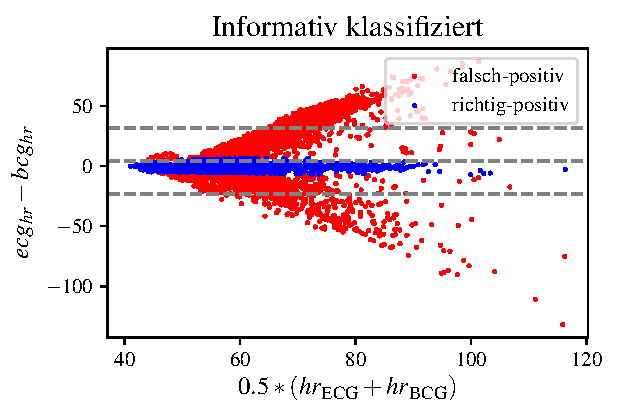
\includegraphics[scale=0.7]{pic/brueser04-bland-altman-inf.pdf}
% 			\caption[$q_{th}=0.4$]{$q_{th}=0.4$}
% 		\end{subfigure}
%    	\begin{subfigure}{.45\textwidth}
%    		\centering
% 			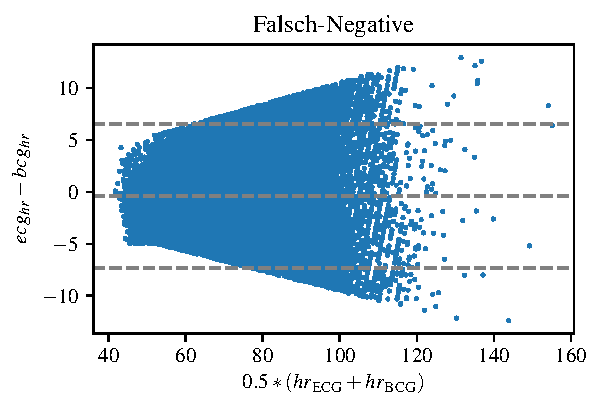
\includegraphics[scale=0.7]{pic/brueser04-bland-altman-fn.pdf}
% 			\caption[$q_{th}=0.4$]{$q_{th}=0.4$}
%		\end{subfigure}
% 	\caption[Verteilung von $E\textsubscript{HR}$ bei den als informativ klassifizierten Segmenten]{Verteilung von $E\textsubscript{HR}$ bei den als informativ klassifizierten Segmenten}
% 	\label{fig:brueser-positives}
% \end{figure}
 
 
 \begin{figure}[H]
 	\centering
		\begin{subfigure}{.45\textwidth}
			\centering
 			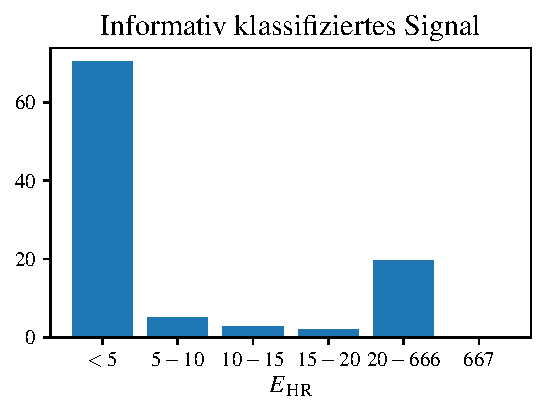
\includegraphics[scale=0.7]{pic/brueser04-positives.pdf}
 			\caption[$q_{th}=0.4$]{$q_{th}=0.4$}
 		\end{subfigure}
    	\begin{subfigure}{.45\textwidth}
    		\centering
 			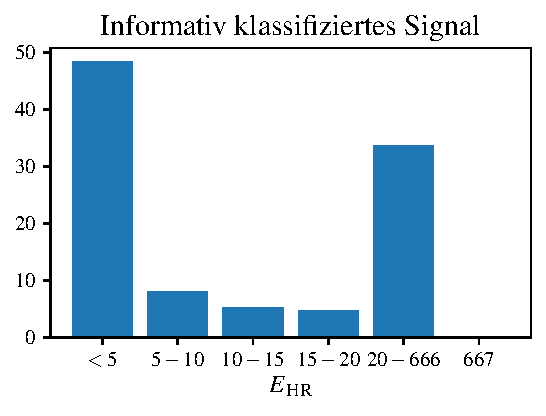
\includegraphics[scale=0.7]{pic/brueser03-positives.pdf}
 			\caption[$q_{th}=0.3$]{$q_{th}=0.3$}
 		\end{subfigure}
 	\caption[Verteilung von $E\textsubscript{HR}$ bei den als informativ klassifizierten Segmenten]{Verteilung von $E\textsubscript{HR}$ bei den als informativ klassifizierten Segmenten}
 	\label{fig:brueser-positives}
 \end{figure}
 
 % TODO: Visualisierung Coverage
 Außerdem wurde untersucht, wie hoch die Coverage unter einem bestimmten Fehler $E\textsubscript{HR}$ auf dem gesamten Signal ist, wenn nur die als informativ klassifizierten Segmente verwendet werden. Hier wird besonders sichtbar, wie niedrig die erreichte Coverage ist. So werden mit $q_{th}=0{,}4$ und $c_{th}=75$ nur 5{,}42\,\% Coverage für $E\textsubscript{HR} < 5$ erreicht werden, obwohl das ganze Signal 32{,}61\,\% enthält. Mit $q_{th}=0{,}3$ und $c_{th}=75$ sind es immerhin 8{,}82\,\%, aber auch das liegt deutlich unter dem tatsächlichen Wert. Die Verteilung ist auch in Abbildung \ref{fig:brueser-coverage} gezeigt.
 
 \begin{figure}[H]
 	\centering
  	\begin{tabular}{l || c | c | c}
 									& insgesamt 		& $q_{th}=0{,}3, c_{th}=75$ & $q_{th}=0{,}4, c_{th}=75$\\\hline
 		$E\textsubscript{HR} < 5$ 	&  32{,}61\,\% 	& 8,82\,\% 					& 5,42\,\%	\\
 		$E\textsubscript{HR} < 10$ 	&  43{,}22\,\% 	& 15,33\,\% 					& 7,39\,\%	\\
 		$E\textsubscript{HR} < 15$ 	&  51{,}66\,\% 	& 20,44\,\% 					& 8,39\,\%	\\
 		$E\textsubscript{HR} < 20$ 	&  59{,}40\,\% 	& 24,60\,\% 					& 9,18\,\%\\
 	\end{tabular}
 	\caption[Coverage unter bestimmten Fehlern $E\textsubscript{HR}$ vor und nach Klassifikation]{Coverage unter bestimmten Fehlern $E\textsubscript{HR}$ vor und nach Klassifikation}
 	\label{fig:brueser-coverage}
 \end{figure}
 
 Alles in allem zeigt sich, dass trotz einer sehr niedrigen erreichten Coverage der Fehler in der Klassifikation verhältnismäßig hoch ist. Dieses Verfahren ist also bei dem hier vorliegenden Signal nicht ausreichend. Wenn $q_{th}$ und $c_{th}$ nicht zu niedrig gewählt werden, kann ein Teil des nicht informativen Signals markiert und somit der Fehler in weiterer Verarbeitung insgesamt reduziert werden. 
 

\subsection{Schwellwerte für Standardabweichung, Minimum und Maximum}

Für das zweite getestete Verfahren werden lediglich zwei Schwellwerte $T_1$ und $T_2$ benötigt, die auf Standardabweichung, Minimum, Maximum und Durchschnitt des Signals beruhen. Die Klassifikation ist ein einfacher Vergleich. \citeauthor{Pino2015} verwenden sehr kleine Fenster, die hier aufgrund fehlender Robustheit der Annotation nicht verwendet werden können.\footcite[]{Pino2015} Stattdessen wird der Algorithmus sowohl auf 10\,Sekunden- als auch 4\,Sekunden-Segmenten getestet, damit sichtbar wird, ob die Segmentlänge einen Einfluss auf das Ergebnis hat.

Die Tests mit beiden Segmentlängen zeigen, dass dieses Verfahren für die in dieser Arbeit untersuchten Daten nicht nutzbar ist, da bei beiden über 95\,\% der Daten als informativ klassifiziert werden, darunter auch Segmente, bei denen $E\textsubscript{HR}$ maximal ist. Weiterführende Evaluation bietet hier keine weiteren Erkenntnisse. Dieses Verfahren ist damit nicht weiter nutzbar.

\subsection{Maschinelles Lernen mittels statistischer Merkmale}

Für das maschinellen Lernen mittels statistischer Merkmale werden die in Kapital \ref{ml-beschreibung} aufgezählten Merkmale extrahiert. Als Bibliothek für die Modelle des maschinellen Lernens wird \textit{scikit-learn}\footcite[]{scikit-learn} verwendet. Da die Daten sich grundlegend von den von \citeauthor{Sadek2016} untersuchten unterscheiden, werden die Hyperparameter der Modelle im Zuge dieser Arbeit erneut optimiert. Bei der dafür durchgeführten Kreuzvalidierung wird wie schon bei der Unterteilung in Trainings- und Validierungsset anhand der Patient*innen-ID geteilt, damit auch diese aussagekräftige Ergebnisse liefert.

Insgesamt zeigen bereits Accuracy und \ac{MAE}, siehe Abbildung \ref{fig:ml-statistical-MAE-Coverage}, eindeutig, dass die Klassifikation mit keinem der Modelle sehr erfolgreich ist. Die Accuracy von im besten Fall 0,57 zeigt, dass die Klassifikation nur minimal besser als reines Raten ist. Teils ist der \ac{MAE} der als informativ klassifizierten Segmente sogar größer als der auf dem gesamten Signal. In der folgenden tiefergehenden Evaluation werden lediglich \ac{RF} und \ac{MLP} betrachtet. Zwar sind die Ergebnisse des \ac{DT} auf einem ähnlichen Nivea, aber da ein \ac{RF} lediglich ein Zusammenschluss mehrerer \ac{DT} ist, ist eine zusätzliche Analyse nicht lohnenswert. 

\begin{figure}[H]
	\centering
 	\begin{tabular}{l || c | c | c | c}
 					& \ac{MAE}	& Coverage		& Accuracy	& Accuracy der Kreuzvalidierung\\ \hline
 		insgesamt 	& 21{,}84	& -				& - 			& -\\
 		annotiert	& 3{,}28		& 43{,}22\,\%	& - 			& -\\ \hline
 		\acs{LDA}	& 21{,}84	& 84{,}81\,\%	& 0{,}49		& 0{,}51\\
 		\acs{SVM}	& 22{,}06	& 88{,}14\,\%	& 0{,}47		& 0{,}55\\
 		\acs{DT}	& 19{,}39	& 47{,}20\,\%	& 0{,}53		& 0{,}52\\
 		\acs{RF}	& 17{,}66	& 44{,}20\,\%	& 0{,}57		& 0{,}52\\
 		\acs{MLP}	& 18{,}41	& 42{,}04\,\%	& 0{,}56		& 0{,}54\\
 	\end{tabular}
 	\caption[Fehler und Coverage der Klassifikation für die verschiedenen Modellen des maschinellen Lernens mit statistischen Merkmalen im Vergleich um gesamten Signal und der Annotation]{Fehler und Coverage für die verschiedenen Modelle im Vergleich zum gesamten Signal und der Annotation}
 	\label{fig:ml-statistical-MAE-Coverage}
\end{figure}

Bei einer ähnlich hohen Coverage wie der Annotation ist der deutlich höhere \ac{MAE} der Klassifikation in falsch-positiven Segmenten begründet. Der Anteil von Segmenten mit einem Fehler $E\textsubscript{HR}$ größer als 20 ist bei beiden Modellen mit ca. 35\,\% ähnlich hoch. Zusätzlich sind 0{,}006\,\% der vom \ac{DT} als informativ klassifizierten Segmente solche, bei den $E\textsubscript{HR}$ maximal ist. Das bedeutet, dass die falsch-positiv klassifizierten Segmente bei beiden Klassifikatoren keine Randfälle sind. Der \ac{MAE} der falsch-negativen Klassifikationen beträgt beim \ac{RF} 3,48 und beim \ac{MLP} 3{,}39, ist also zwar leicht höher als der \ac{MAE} aller informativen Segmente, aber nicht relevant. Auch bei diesen handelt es sich also nicht um Randfälle.
 	
 \begin{figure}[H]
 	\centering
		\begin{subfigure}{.45\textwidth}
			\centering
 			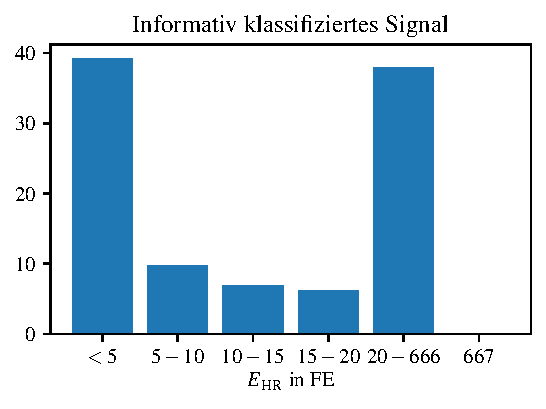
\includegraphics[scale=0.7]{pic/rf-statistical-positives.pdf}
 			\caption[RF]{RF}
 		\end{subfigure}
    	\begin{subfigure}{.45\textwidth}
    		\centering
 			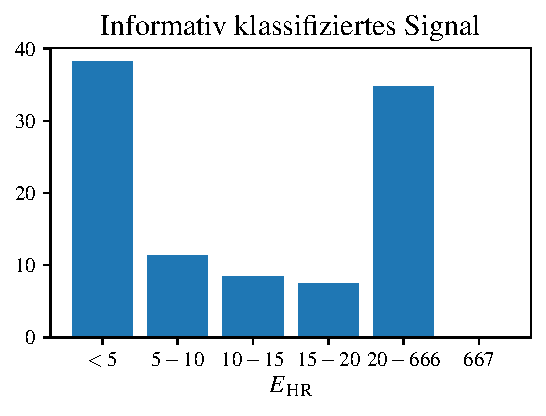
\includegraphics[scale=0.7]{pic/mlp-statistical-positives.pdf}
 			\caption[MLP]{MLP}
 		\end{subfigure}
 	\caption[Verteilung von $E\textsubscript{HR}$ bei den als informativ klassifizierten Segmenten]{Verteilung von $E\textsubscript{HR}$ bei den als informativ klassifizierten Segmenten}
 	\label{fig:ml-statistical-positives}
 \end{figure}
 
 Auch für diese Modelle wird untersucht, wie hoch die Coverage unter einem bestimmten Fehler $E\textsubscript{HR}$ bei der Betrachtung des als informativ klassifizierten Signals auf dem ganzen Signal ist. Auffallend ist, dass die Werte knapp halb so hoch wie die tatsächliche Coverage sind. Das zeigt ergänzend zu der gemessen Accuracy, dass ca. die Hälfte der Segmente, unabhängig von ihren tatsächlichen Qualität, als informativ klassifiziert werden.
 
  \begin{figure}[H]
 	\centering
  	\begin{tabular}{l || c | c | c}
 									& insgesamt 		& RF			& MLP\\\hline
 		$E\textsubscript{HR} < 5$ 	&  32{,}61\,\% 	& 17,35\,\%		& 16,07\,\%	\\
 		$E\textsubscript{HR} < 10$ 	&  43{,}22\,\% 	& 22,20\,\% 		& 20,82\,\%	\\
 		$E\textsubscript{HR} < 15$ 	&  51{,}66\,\% 	& 25,92\,\% 		& 24,34\,\%	\\
 		$E\textsubscript{HR} < 20$ 	&  59{,}40\,\% 	& 29,23\,\% 		& 27,45\,\%\\
 	\end{tabular}
 	\caption[Coverage unter bestimmten Fehlern $E\textsubscript{HR}$ vor und nach Klassifikation]{Coverage unter bestimmten Fehlern $E\textsubscript{HR}$ vor und nach Klassifikation}
 	\label{fig:ml-statistical-coverage}
 \end{figure}
 
 Insgesamt zeigt sich, dass die Klassifikation mittels statistischer Merkmale bei vorliegenden Daten und Annotation nicht erfolgreich ist. Zwar wurden auf anderen Daten sehr gute Ergebnisse erreicht, aber es bestätigt sich die Vermutung, dass sich dies, vermutlich aufgrund der unterschiedlichen Aufnahmesituation der Daten und der nicht aussagekräftigen Validierung der Ergebnisse für die im Paper untersuchten Daten, nicht übertragen lässt. 
 
\section{Analyse der Merkmale}

Obwohl keines der Verfahren für die vorliegenden Daten zufriedenstellende Ergebnisse erzielt, ist besonders bei den Modellen maschinellen Lernens interessant, welchen Einfluss und welchen Informationsgewinn die jeweiligen Merkmale haben bzw. liefern. Aus diesem Grund wird im Folgenden eine explorative Datenanalyse durchgeführt.

Zunächst wird betrachtet, ob die Merkmale untereinander und mit $E\textsubscript{HR}$ und der Annotation korreliert sind. Da die Merkmale das Segment gemeinschaftlich statistisch beschreiben ist eine hohe Korrelation untereinander erwartet und zeigt sich auch. Eine Ausnahme bilden Kurtosis, Mittelwert und Schiefe. Außerdem zeigt sich bei der Betrachtung des in Abbildung \ref{fig:corr-heatmap-statistical} abgebildeten Korrelationsdiagramm, dass die Korrelation zu $E\textsubscript{HR}$ und der Annotation nicht signifikant ist. Auch bei paarweiser Visualisierung zeigt sich, dass sich anhand keines untersuchten Merkmalspaares informative von nicht informativen unterscheiden lassen.

\begin{figure}[H]
	\centering
	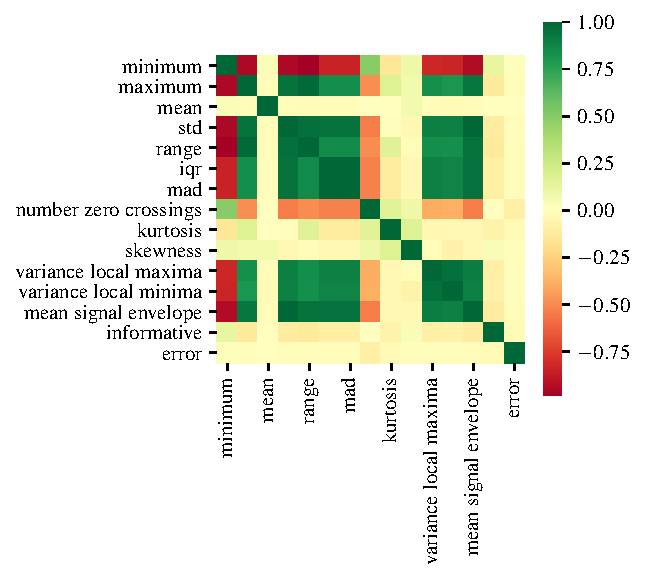
\includegraphics[scale=0.85]{pic/corr-heatmap-statistical.pdf}
	\caption{Korrelationsdiagramm der statistischen Merkmale, $E\textsubscript{HR}$ und der binären Annotation}
	\label{fig:corr-heatmap-statistical}
\end{figure}

Da die Visualisierung hochdimensionaler Daten schwierig ist und auch Modelle maschinellen Lernens bei einer hohen Merkmalszahl aufwändiger zu trainieren sind, wurde ebenfalls untersucht, wie sich die Daten bei einer Transformation in einen zweidimensionalen Raum verhalten. Untersuchte Transformationen umfassen sowohl unüberwachte Verfahren wie \ac{PCA} mit verschiedenen Kernel als auch überwachte Verfahren wie eine Dimensionsreduktion mit einer \ac{LDA}. Auch die transformierten Daten lassen sich nicht voneinander trennen, wie auch in Abbildung \ref{fig:dim-red-statistical} beispielhaft für eine \ac{PCA} mit linearem Kernel gezeigt ist.


 \begin{figure}[H]
 	\centering
 	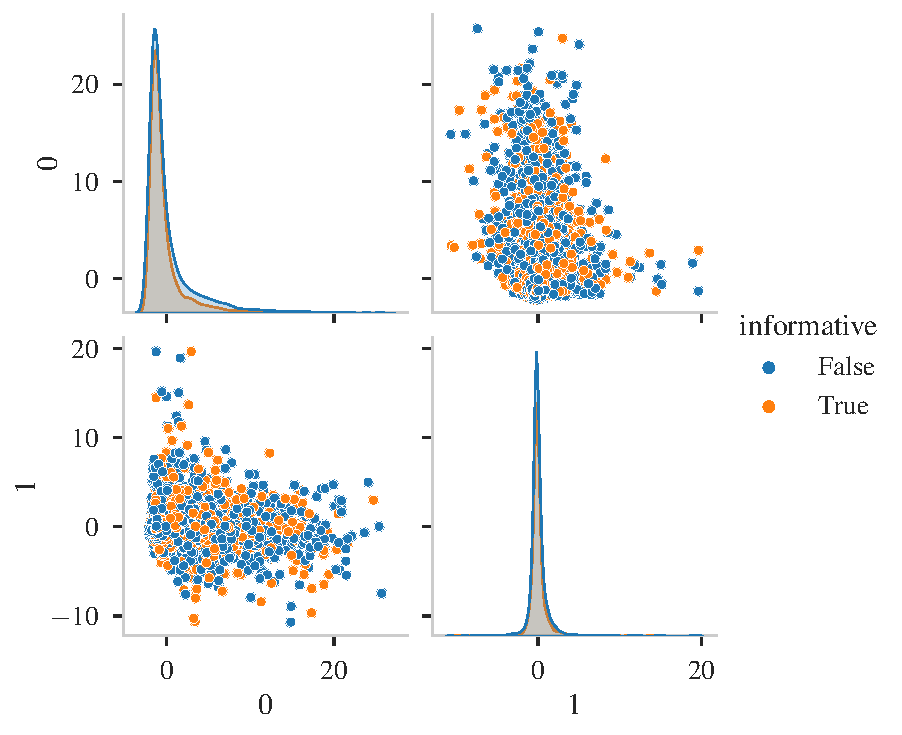
\includegraphics[scale=0.6]{pic/statistical-pca-lin.pdf}
	\caption{Dimensionsreduktion der statistischen Merkmale mit einer \ac{PCA} mit linearem Kernel}
	\label{fig:dim-red-statistical}
\end{figure}

Weiteren Einblick ermöglicht die Analyse des \ac{RF}, da bei diesem ermittelt werden kann, wie wichtig die einzelnen Merkmale jeweils für die Entscheidungsfindung sind. Das Ergebnis zeigt, dass der Durchschnitt des Signals deutlich weniger Einfluss als die anderen betrachteten Merkmale hat. Die Schiefe (skewness) und die Anzahl der Nulldurchläufe sind, wie in Abbildung \ref{fig:rf-statistical-importances} zu sehen, die beiden wichtigsten Merkmale. 

\begin{figure}[H]
	\centering
	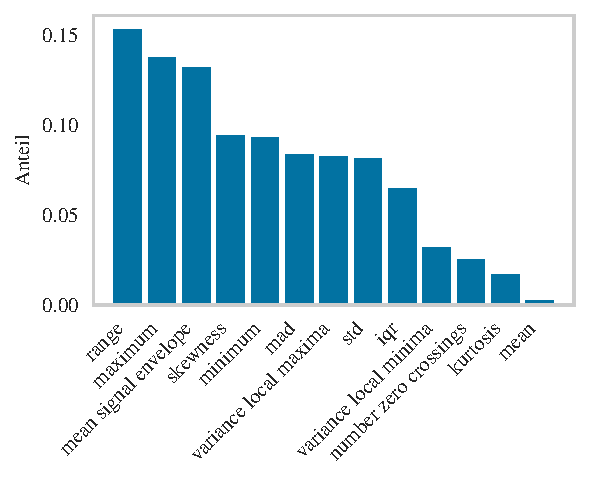
\includegraphics[scale=0.9]{pic/rf-cl-statistical.pdf}
	\caption{Wichtigkeit der Merkmale für den \ac{RF}-Klassifikator}
	\label{fig:rf-statistical-importances}
\end{figure}

Anhand der statistischen Merkmale kann also keine Klassifikation vorgenommen werden. Vermutlich sorgt die große Variation der in Betten aufgenommenen \ac{BKG}-Signale dafür, dass sich die Signale nicht statistisch verallgemeinern lassen. Auch die reine Betrachtung der Ähnlichkeit der Intervallschätzer ist nicht ausreichend. Es müssen also andere Merkmale gefunden werden, die allein oder ergänzend zu den bereits betrachteten eine Aussage zu der Signalqualität ermöglichen.